% !TEX program = xelatex
\documentclass[11pt,a4paper]{article}
\usepackage{polyglossia}
\usepackage{fontspec}
\usepackage{subfig}
\usepackage{url}
\usepackage{hyperref}
\usepackage[round]{natbib}
\usepackage[font=small]{caption}
\usepackage{amsmath}
\usepackage[usenames,dvipsnames,svgnames,table]{xcolor}

% natbib link joining; somewhat breaks \citep, \citept
\makeatletter
\renewcommand\hyper@natlinkbreak[2]{#1}
\makeatother

\usepackage{geometry}
\geometry{%
	includeheadfoot,
	margin=1in
}

\def\TODO{{\bf ??? }}

\title{Argus: Deciding Questions about Events \\ (working paper v1.3pre2)}
\author{Petr Baudiš, Silvestr Stanko \\ Ailao}

\begin{document}
\maketitle

\begin{abstract}%
	We consider the problem of reliably answering yes/no questions
	about events based on news sources in settings of the Argus QA
	system and the Syphon question pre-validator.
	We give a brief overview of the relevant state-of-art methods
	in the academic field of Natural Language Processing,
	requirements for building a solid state-of-art system
	and difficulties we may anticipate on the road ahead.
	Based on this, we propose a basic architecture of the Argus
	system, a roadmap to achieve baseline performance, and a basic
	version of the Syphon system.
\end{abstract}

\vspace{3ex}

The task of the \textbf{Argus} system within \textsc{Augur}
is to automatically analyze and answer
questions by users that relate to future events.  This is supposed
to be an alternative to the manual answering process done by humans,
or an augmentation that pre-suggests answers and provides gathered
evidence for a final human decision, allowing the process to scale
up greatly.  Another important \textsc{Augur} module tightly
coupled to Argus is \textbf{Syphon} which provides an interactive
user interface when asking a question, including auto-completion,
auto-validation and possibly a template system, with the aim to
ensure clarity and unambiguity of questions and permit reliable
Argus operation.

Our team at the Ailao startup, based at the 3C Group FEE CTU,
is composed of people working at the boundary of academic and commercial
sector and with a history of projects that involve
various aspects of Natural Language Processing ---
information retrieval, web scraping and information extraction,
deep learning, and, most prominently in this context, question answering.
Our flagship project is the YodaQA system for answering factoid questions,%
\footnote{\url{http://ailao.eu/yodaqa}}
but we also built other NLP systems aiming at some level of language understanding,
like automatic tagging of newsreel messages
or answering multiple-choice logical entrance exam type questions.

A natural question is whether we could simply apply our YodaQA system
on this task.  However, while there are some common analysis elements,
generating factoid answers is programatically quite a different task
from deciding whether a sentence is correct or incorrect,%
\footnote{A baseline support for answering yes / no questions is currently
under development within YodaQA as a student internship project, but it is
not finished yet and not meant to be highly reliable at this point.
The initial proposed method is at
\url{https://github.com/brmson/yodaqa/blob/f/textent/doc/ENTAILMENT.md}
but the difference from our scenario is that we are answering questions
on top of a fixed knowledge base, mainly structured one, rather than an
evolving news stream.  The baseline techniques are also so simple that
reusing implementation wouldn't help that much --- but reusing experience
definitely will.}
as we explain in more detail below.
We believe the most efficient approach to take for a prototype is thus
to build a system from scratch, reusing mainly our expertise and possibly
some isolated external components (e.g.\ database interfaces or NLP annotators).

The rest of the paper is structured as follows.
In Sec.~\ref{qaml}, we rehash what does it involve to build a Natural Language Processing
system that uses machine learning and is rigorously developed and measured.
In Sec.~\ref{ynml}, we look at the current scientific concepts that relate
to the yes/no QA task at hand, and at their performance.
In Sec.~\ref{structure}, we explore the yes/no QA task in more detail,
identifying different types of questions and how to tackle each.
As a corollary, we explain how to sort the easy from the difficult
even before attempting an answer in Sec.~\ref{syphon}.
We sketch the system and its main concrete strategies based on these
ingredients in Sec.~\ref{system}.
Lastly in the Sec.~\ref{infra}, we give an overview of
the most essential part of the system --- the infrastructure
that collects and manages our data, runs the experiments and interacts with the user.

\section{QA System in the Machine Learning Context}
\label{qaml}

When building an NLP system that uses machine learning components,
we need a rigorous way to (i) train these components, and (ii) evaluate
the system performance.

Our NLP system is a \textit{classifier}, i.e.\ a program that takes
a sentence (and a large knowledge base) and classifies it as either
true or false.  The typical approach in such a scenario is building
a \textit{gold standard} dataset --- a set of questions, each annotated
with the correct answer (yes, no, unknown) and an accompanying knowledge
base that should, on its own, lend support to deciding these questions.%
\footnote{With a large enough knowledge base, this issue tends to vanish,
of course.}

In general, the bigger the dataset, the better.  Commonly used datasets
range in size from the low hundreds%
\footnote{E.g.\ the \textit{Curated TREC QA Track Dataset} \url{https://github.com/brmson/dataset-curated-factoid/}}
to the tens of thousands%
\footnote{E.g.\ the \textit{Large Movie Review Dataset} \url{http://ai.stanford.edu/~amaas/data/sentiment/}}
(of questions, statements, queries)
but we can certainly grow the dataset as needed and we will be able to identify
insufficient dataset size as a possible improvement factor during development.
We should start with at least 100 questions for initial evaluation of our
baseline.

These questions are further split --- at the very least, to a \textit{training}
set and a \textit{testing} set (even finer splits are often desirable
with enough questions available).
To train even simple machine learning models, we should try hard to get
at least 300 questions, but to train some more advanced models, we need
to aim at figures like 6000 questions.

To get the dataset, the simplest option is to hire low-paid virtual assistants
to build it.  Aside of using common employment platforms, Amazon runs a
so-called Mechanical Turk service that allow humans to be employed easily
for these kinds of tasks.  Finally, it might be possible to build the dataset
semi-automatically by using some clever approaches --- this makes it easy
to build a large dataset, but presents the danger of noise (non-sensical questions
or wrong reference answers) and drifting off from realistic questions the
users will pose.  It would be an interesting problem / milestone on its own,
but something we might have to tackle.

Many of the models need another kind of dataset as well --- pairs of question
and news sentence that are annotated by whether the sentence carries the yes/no
answer for the question.  However, from a purely question-based dataset,
generating a medium-quality dataset like this should be straightforward,
and reviewing predefined annotations by humans is much easier and faster
than creating the annotations in the first place.

The main criterium for evaluating our system is obviously \textit{accuracy},
that is the percentage of questions our system gets right.  However, this
number does not capture questions where the system ``gives up'' and says
unknown; one possibility is to use a harmonic average of (i) the percentage
of questions the system gets right when it decides to answer, and (ii) the
percentage of questions the system decides to answer.%
\footnote{This combined percentage is called \textit{F1 score} in machine learning jargon.}
We can always change the threshold of confidence the system uses to decide
whether to answer to keep the accuracy of answered questions at the minimum
target score of 95\%, the caveat is that the system may refuse to answer almost
all questions at that point; therefore, this average metric is a better
option for judging the system's performance.

Performance evaluation in the machine learning context has two clear limitations
that we are not sure how to overcome right now.  First, it is not clear how to
effectively evaluate Syphon performance when users are repeatedly adjusting
their queries to force them through; we'll come back to this below.
Second, we assume a \textit{non-adversarial scenario} where user questions
are expected to be unbiased and users are not actively trying to trick the system;
this assumption is not realistic, but we are not aware of any good answers science
has to this problem.  Out-of-the-loop safeguards like random manual review,
adaptive Syphon or large-scale consensus of diverse automata might be required.
Another possibility is that a group of ``white hat'' users will counter-analyze
trending questions for possible flaws of this nature and natural balance will
emerge in the ecosystem --- the motivation of these users being reputation and
credentials (user rating might be an excellent base for getting hired as a
proprietary analyst), or even bounties for bad questions.

\section{Machine Learning for Answering Yes/No Questions}
\label{ynml}

When considering the relevant state-of-art in Machine Learning (ML) and
Natural Language Processing (NLP), we will first give a short overview
of the recent advances in general natural language processing techniques,
then consider the state-of-art in all the specific areas pertaining to our question
answering task.

\subsection{Vector Embeddings}

Recent progress in NLP has been marked mainly by the proliferation of
so-called \textit{vector embeddings}, the most popular being called
\textit{word2vec}.  This approach stems from the so-called \textit{distributional semantics}
hypothesis, which posits that we can derive meanings of words purely
from the context they tend to appear in.  Therefore, each word is
associated with a list of $n$ real numbers (i.e.\ coordinates of
an $n$-dimensional vector) and these numbers are derived automatically
just from the context the words appear in.%
\footnote{The \textit{word2vec} method uses an idea called \textit{multi-task learning}
	which may be useful for us as well --- we try to learn
	some easy-to-specify task and then we re-use the same model to
	solve some much harder problems.  Here, the $n$ real numbers
	come out from training a classifier that predicts the most likely
	next words to come given a context of (say, 100) preceding words;
	this so-called \textit{language model} task is useful e.g.\ in
	speech recognition or OCR.}
The interesting property is that the automatically assigned numbers
exhibit semantic properties in how they relate between words.
For example, if we do arithmetics on these word vectors and try
to compute e.g.\ $king + (woman - man)$, the nearest vector we reach
is $queen$, i.e.\ the gender transition is represented by an arrow
in our vector space (Fig.~\ref{fig:w2vg}).
Fig.~\ref{fig:w2ver} shows how relationships between adjectives are represented
while Fig.~\ref{fig:w2vc} shows mappings between coordinates of countries
and their capitals.  Let us emphasize again that these coordinates were
determined purely based on the context of the words (in Wikipedia or
millions of news articles); the system did not have any extra information
or databases available.

\begin{figure}[ht]
	\centering
	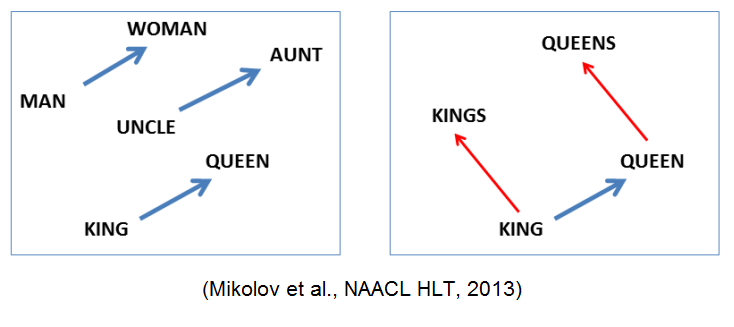
\includegraphics[width=10cm]{kingqueen.png}
	\caption{Semantic relationships between words as arrows in the vector space. \cite{WordVecLingReg}}
	\label{fig:w2vg}
\end{figure}

\begin{figure}[p]
	\centering
	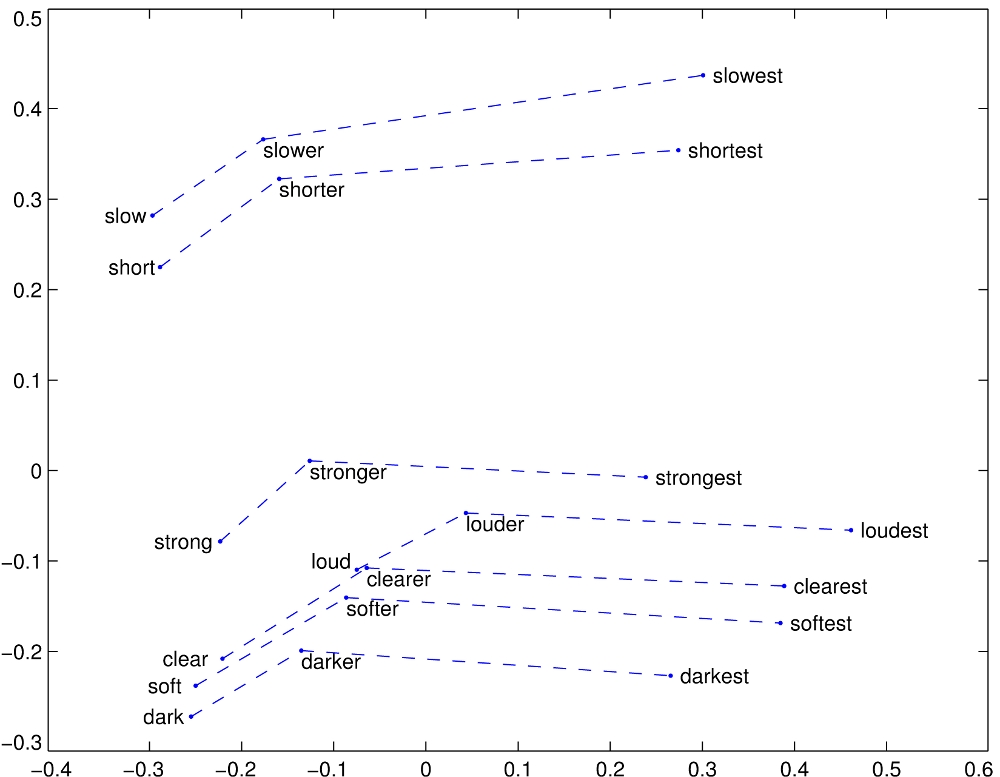
\includegraphics[width=10cm]{comparative_superlative.jpg}
	\caption{Semantic relationships between superlative adjectives as represented in the vector space.
		This is a 2D projection of the high-dimensional space that is designed to well preserve relative positions of the shown entities
		(so-called t-SNE 2D).
		\cite{Glove}}
	\label{fig:w2ver}
\end{figure}

\begin{figure}[p]
	\centering
	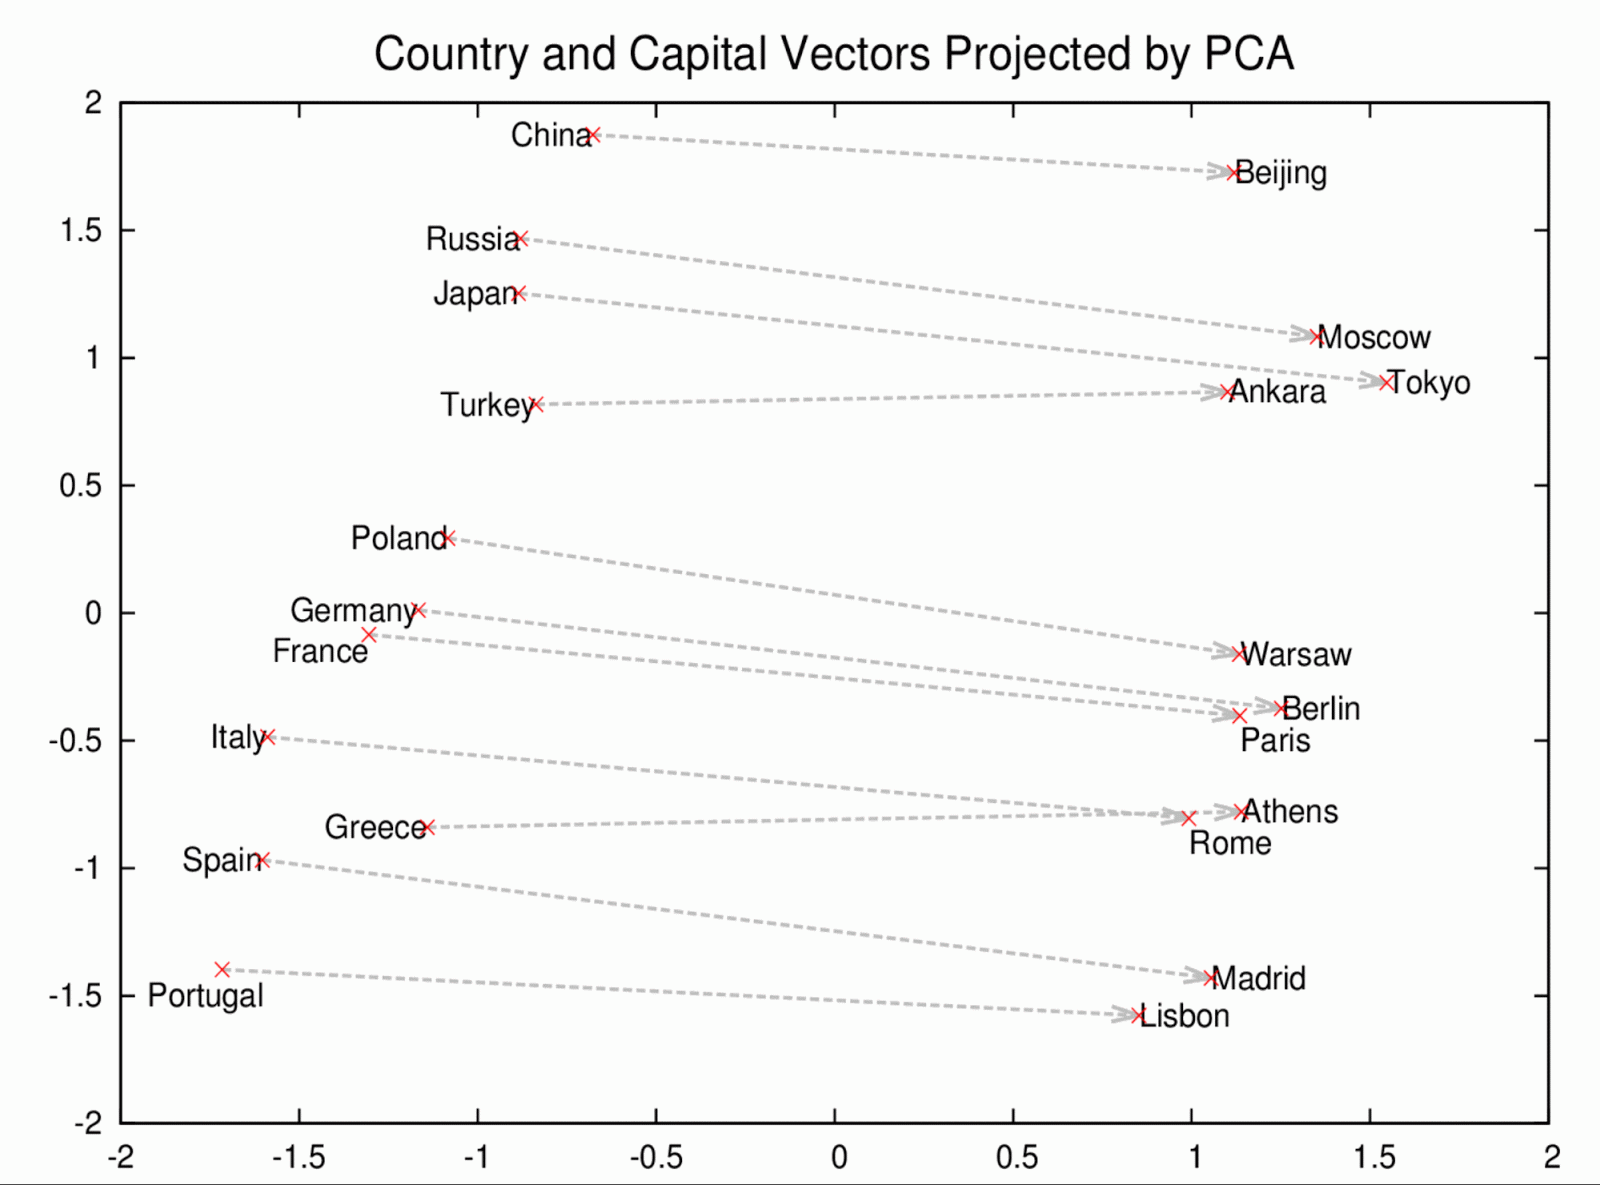
\includegraphics[width=11cm]{capitals.png}
	\caption{Mappings between countries and capitals, acquired entirely from the typical context of the respective words.
	This is again a 2D projection of the high-dimensional space, this time obtained by a PCA dimensionality reduction technique.
	\cite{DistReprComp}}
	\label{fig:w2vc}
\end{figure}

A lot of the current research focuses on the best ways to build up
vector representations of whole sentences and documents --- ranging
from simple averaging \citep{CNNSentClass,DefGen} (successful baselines)
to recurrent neural networks \citep{LISA,ShowAndTell}.
Many applications that rely on semantic understanding of word nuances
are popping up; this method became state-of-art for machine translation
\citep{LISA}, automatic image captioning \citep{ShowAndTell} and specific
types of question answering \citep{QANTA,DefGen,ReadAndComprehend}%
\footnote{The demo at \url{http://45.55.181.170/defgen/} is nice.}.
One open problem is efficient composition of vector embeddings for
common words with entities like numbers or proper names.

\subsection{NLP for Yes/No Questions}

The standard NLP problem which is closest to answering yes/no questions
is the so-called \textit{Recognizing Text Entailment} (RTE) task.
In the standard formulation,
we have a paragraph of context and a phrase that either is or isn't
\textit{entailed}, i.e.\ can be decided to be true just based on the context.
The most prominent effort in this area is probably the
\textsc{Excitement EOP} academic project,%
\footnote{\url{http://hltfbk.github.io/Excitement-Open-Platform/}}
which is a full-fledged
RTE pipeline in Java that implements several algorithms
in a common framework.
Typical state-of-art RTE algorithms work on the principle of parse tree
alignment --- grammar dependency tree of the hypothesis and each context
sentence is compared and we try to learn which changes in the tree might
keep entailment.
But as the RTE problems are quite hard and practical applications are limited,
this is not a very lively area of research per se.

In the RTE field jargon, the Argus task is to detect whether either the question or
its negation is entailed from a given text article.  This involves
a mechanism to focus on the relevant parts of the article (if any)
and some sort of semantic analysis of these parts to determine
equivalence.
However, we argue that our task significantly differs from
the industry-standard benchmarks.  A few examples are listed in Fig.~\ref{fig:rte3}
(more examples include answering ``text comprehension'' problems from
English SAT exams%
\footnote{An example of this is: \url{http://nlp.uned.es/entrance-exams/}.})
and they demonstrate that the main focus of the RTE field is to enhance
deep computer understanding of written text and often the questions
require non-trivial inference from information-rich sentences.
Of course, this is a task a perfect, Syphon-less Argus type system
would eventually need to solve too, but our focus right now is on a much
easier task, where often many news headings will literally already contain
the answer we need.  In contrast to RTE, where the contextual paragraph is
typically a short snippet, our main focus is filtering the news source for
the relevant passages.

\begin{figure}
	\footnotesize
	\textbf{Context:} The sale was made to pay Yukos' US\$ 27.5 billion tax bill, Yuganskneftegaz was originally sold for US\$ 9.4 billion to a little known company Baikalfinansgroup which was later bought by the Russian state-owned oil company Rosneft. \\
	\textbf{Hypothesis:} Baikalfinansgroup was sold to Rosneft.

	\vspace{2ex}

	\textbf{Context:} US Steel could even have a technical advantage over Nucor since one new method of steel making it is considering, thin strip casting, may produce higher quality steel than the Nucor thin slab technique. \\
	\textbf{Hypothesis:} US Steel may invest in strip casting.

	\vspace{2ex}

	\textbf{Context:} The 'Club of Rome' was an appalling Joy Division soundalike band playing in Canberra, Australia in the early 1980's. They were foul, really. Boring, pretentious bunch of shore-starers who struggled to string a tune together, while all the while revelling in the reflected glory of late greats like the Birthday Party. Oh yeah, and they have the same name as some global think tank that deals with a variety of international political issues. \\
	\textbf{Hypothesis:} The 'Club of Rome' is a global think tank that deals with a variety of international political issues.

	\caption{Typical RTE pairs from academic datasets, mainly the ERT-3 challenge.}
	\label{fig:rte3}
\end{figure}

With this in mind, let us cover some recent successes mainly of
the vector embedding methods in some of the NLP fields related
to understanding of written text, but less demanding than the
full RTE task.  Let us cover a few popular benchmarks:

\begin{itemize}
	\item \textbf{Sentiment Analysis:} One of the chief benchmarks of
		language understanding, classifying texts (e.g.\ product
		reviews) as either positive and negative --- there are
		abundant datasets, eminent commercial applicability,
		the problem is very easy to phrase and judge, and yet
		simple models fail to solve it effectively.%
\footnote{Consider this utterance with a lot of positive words:
		\textit{This movie was actually neither that funny, nor super witty.}}
		The state-of-art (as far as we know) are the Recursive
		Neural Tensor Networks that model grammar-dependent
		transformations of vector embeddings, with
		85.4\% sentences correctly classified as positive or
		negative on the standard dataset. \citep{SentimentRNTN}
		A major relevance of this area for us is that detection
		of long-range negations or even irony is important in
		sentiment analysis.

	\item \textbf{Question Answering:} The problem we are ourselves
		tackling is question answering, however the primary focus
		there is the process of \textit{generating} facts while
		here we are in the business of \textit{verifying} them.
		Such a component would be obviously also useful in
		a question answering system, but e.g.\ in our \textit{YodaQA}
		system, we do not have such a (working) component yet.
		IBM Watson DeepQA system (famous from the Jeopardy! competition)
		has such a component described in \citep{WatsonEvidence};
		they propose also several simple techniques we plan to
		use as our baselines.

		Nevertheless, the question answering task is large and
		consists of many specific sub-tasks.  Let us detail two
		that would be relevant for us.

	\item \textbf{Question Type Classification:} This task can serve
		as a demo of state-of-art capability to classify a sentence
		into a specific category, in this case whether the question
		is, say, about a number or an entity.  State-of-art approaches
		(93.2\% accuracy)
		include neural networks based on vector embeddings \citep{QtcDCNN}.
		We are experimenting with some approaches in the YodaQA
		context too.%
\footnote{\url{https://github.com/brmson/question-classification/}}

	\item \textbf{Answer Sentence Selection:} A significant portion
		of our problem will be isolating news articles
		and sentences relevant to our questions in large swathes
		of irrelevant data.  The sentence selection sub-task is
		about identifying sentences that bear an answer to the
		given question.%
\footnote{This is a relatively hard problem; the
		classifier, given \textit{What does the Peugeot company manufacture?}
		must select \textit{Peugeot and Rover last month ended an agreement under which Rover distributed Peugeot cars through its dealers in Japan.}
	but reject \textit{Renault and Peugeot are getting less integrated and becoming primarily designers and assemblers.}}
		The state-of-art method \citep{Yu2014Deep} uses vector embeddings
		and when sorting sentences by relevance, achieves a mean rank
		of about 1.2.%
\footnote{To clarify, this is a reciprocial of Mean Reciprocial Rank.}
		We have already built our own implementation of this method
		which reproduces the results and is directly applicable
		in Argus, we believe.%
\footnote{\url{https://github.com/brmson/Sentence-selection}}
		The downside is that we would need a dataset which has
		each sentence manually labelled by whether it answers
		the posed yes/no question.

\end{itemize}

To conclude, the yes/no question answering problem in a scenario that
would make it easily applicable to Argus has been left almost untackled
in the literature.  However, several recent benchmarks in related areas
highlight some techniques which should be highly successful on our task.
The state-of-art algorithms often involve vector embeddings of words,
the caveat of which is the requirement of an extensively annotated
data set, e.g.\ using Mechanical Turk or a hybrid partially automated
approach.

\section{Structure of Our Problem}
\label{structure}

\begin{figure}
\begin{verbatim}
Did Hillary Clinton become President?
Did Scott Walker become US President?
Did Martin O’Malley become US President?
Was Obamacare dismantled by the Supreme Court?
Was Saudi Arabia’s monarchy dethroned in a coup d’etat?
Did Iran test detonate a nuclear bomb?
Did Israel attack Iran?
Did Germany ban the PEDIGA movement?
Did the US dollar collapse by at least 50%?
Did the euro collapse another 50%?
Did Germany abandon the euro?
Did the EU slide into a new recession?
Was a miracle cure for diabetes discovered?
Did a real blizzard lead to power cuts for more than 10 million Americans?
Did Sears declare bankruptcy?
\end{verbatim}
	\caption{Sample questions as provided by the \textsc{Augur} team.}
	\label{fig:sampleq}
\end{figure}

Clearly, not all yes/no questions are created equal:
Some are easy to understand; others are hard.
For some, many news results will carry an answer; others will produce just a smidgen of mentions in the knowledge base.
Some are quantitatively unclear and answers might be triggerred by published subjective opinions.
Let us explore what these distinctions mean,
since recognizing them and rejecting answering
the hard questions outright is our key to achieving a high level of precision.
Fig.~\ref{fig:sampleq} contains a list of sample questions (forward-looking as of now).

Let us group the questions into several classes in terms of how easy to automatically judge they are:

\begin{itemize}
	\item Clear-cut questions: \textbf{Did X Y become President?},
		\textbf{Did Iran test detonate a nuclear bomb?},
		\textbf{Did Germany ban the PEDIGA movement?}

		These should be generally easy to parse by Syphon
		and to answer unambiguously from news sources.

	\item Fuzzy-matching questions: \textbf{Was Saudi Arabia’s monarchy dethroned in a coup d’etat?}
		\textbf{Did Germany abandon the euro?},
		\textbf{Did Sears declare bankruptcy?}

		These are about unambiguous facts and should pass Syphon,
		but simple text matching strategies might fail when
		answering the question - the system needs to match
		``revolution'' to ``dethroned in a coup d'etat'',
		many news titles would use ``leave the eurozone''
		instead of ``abandon the euro'' and ``declare bankrupcy''
		is the same as e.g.\ ``go bankrupt''.

		Based on results like \citep{DefGen,QANTA},
		we can predict that many of the simpler paraphrases
		would be covered by vector embeddings%
\footnote{There is also a Wordnet dictionary that covers many synonymic relationships of individual words, but extending it to verb/noun combinations is less trivial.}
		but this is unlikely to solve the ``abandon the euro''.
		We can either rely on stricter Syphon
		(we could suggest manually created templates like
		``becomes $X$'' and ``stops being $X$''
		with regard to a knowledge base attribute),
		or simply hope that the news sources scanned will use so
		much variation in the phrasing of what happened that the particular phrasing used in the question
		(or something fairly close to it involving close synonyms)
		will still appear often enough; the alpha prototype
		should shed more light on this.

		Also, another tricky part is that \textbf{Sears} is the name
		of many legal entities; do we mean the department store
		chain, \textbf{Sears Holdings} or some sister company?
		However, Syphon can catch ambiguous references like this.

	\item Questions requiring inference: \textbf{Did the US dollar collapse by at least 50\%?},
		\textbf{Did the euro collapse another 50\%?},
		\textbf{Did a real blizzard lead to power cuts for more than 10 million Americans?}

		Answering these questions with simple text matching
		is unlikely to produce any results.  Syphon shouldn't
		be able to decompose this question to simple elements
		and relationships between these and so shouldn't let
		these questions pass through.

		Of course, in the whole-system perspective this means
		that the Syphon will instead
		prompt the user, ask for more detail and
		eventually let a sufficiently precise question on this topic through.

	\item Subjective questions: \textbf{Was Obamacare dismantled by the Supreme Court?},
		\textbf{Did Israel attack Iran?},
		\textbf{Did the EU slide into a new recession?},
		\textbf{Was a miracle cure for diabetes discovered?}

		These questions are particularly tricky as filtering
		them with Syphon may be problematic.  Entity X attacking
		entity Y seems quite unambiguous and well-defined.
		On the other hand, the definition of ``attack'' may
		vary widely\footnote{Israel is a good example as the country is known for executing military and intelligence operations covertly and avoiding admission of involvement.} --- from the bombing of a specific site
		to a full-scale military attack.

		We don't have a good solution to this class of questions,
		except warning users that the act of ``dismantling''
		simply means that enough commentators consider the court
		judgement to be this, the same with ``recession'' or what
		is a ``miracle cure'' (we already have several, or none).
\end{itemize}

Aside of questions posed, another important aspect is what data sources
to use for answering them.  One natural idea which we are working
with from the beginning is scanning news feeds from a variety of reputable
news sites and mining answers from natural text.
However, as an alternative, we could leverage collaboratively maintained
databases.  The most prominent of these is now WikiData, which is becoming the
base of many infoboxes at Wikipedia and follows a well-defined ontology (semantic structure).
We would have to establish some trustworthiness metrics (i.e.\ consider
only high-profile concepts and require the value to be unchallenged in
the database for long enough), but the advantage would be a fairly clear
signal for our system, e.g.\ in the form of clearly valued \textit{currency}
property for the \textit{Germany} entity.

\section{How Can We Know What We Know?}
\label{syphon}

The initial phase of the Argus system needs to be the Syphon sub-system
which carries the role of building up a semantically rich question
representation from the natural language input, rejecting answers where
such a representation cannot be unambiguously built, and providing
some sort of templating and/or auto-completion capabilities for partial
questions.  Even when a representation is built and passed, an important
aspect for trustworthiness of the system is that the representation is
shown (in user-friendly form) to Argus users as a feedback and a clear
signal of how the system will decide the answers.

To maintain a high precision level of answers, the Syphon system should be
conservative about the questions it allows.  For the baseline system,
in light of the analysis of question classes above,
we want to propose a simple Syphon which scans the question
for named entities%
\footnote{\textit{Named entity} in NLP parlance is something that is
	not a plain English word carrying meaning, but e.g.\ a proper
	name or a numerical value (date, monetary amount, \dots).
	There exist specialized scanners that extract named entities
	of specific types; as a simple baseline, we may consider
	all strings that are titles of Wikipedia articles (or redirects,
	that is essentially unique aliases).  For example
	\textit{Hillary Clinton} and \textit{President of the United States}
	both are titles of such articles.}
and verbs which describe clear relationships
and verifies that no words without an assigned role remain
in the question.  This should keep a fair share of the sample questions
covered and with a clear interpretation.
Fig.~\ref{fig:syphon} shows a simple visual concept of the initial Syphon.

\begin{figure}[ht]
	\centering
	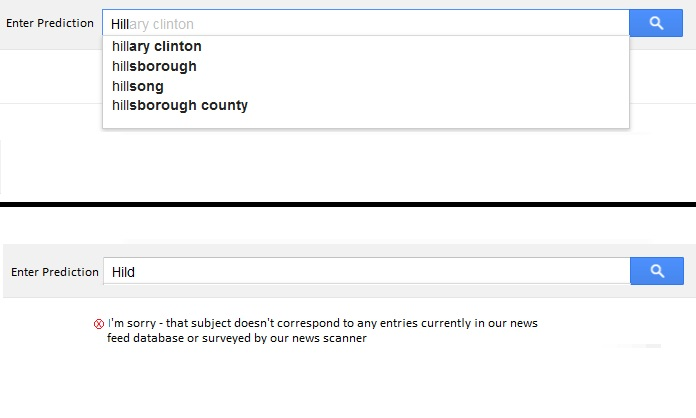
\includegraphics[width=14cm]{syphon_ss.jpg}
	\caption{A visual sketch of Syphon auto-completion aspect.}
	\label{fig:syphon}
\end{figure}

\section{A Concrete Proposal}
\label{system}

Based on the analysis above, let us summarize and outline a particular
proposal for a baseline system:

\begin{itemize}
	\item Syphon module that detects and requires named entities (enwiki titles, dates, \dots) and verbs, rejects if anything extra is present.
	\item Pre-processed question is transferred from Syphon to Argus back-end.
	\item News titles (and possibly article texts, structured databases) are scanned for relevant data, entailment (yes, no, unknown) is modelled for each.
	\item Relative entailment counts (normalized by general frequency of the named entity in the souces) are used to estimate probability.
	\item The output is accompanied with a justification --- summary of evidence for or against the system decision.
\end{itemize}

As the very first knowledge base, we may acquire a number of articles
from a defined past period from The Guardian (reputable UK newspaper)
as they have an appealing API for these purposes.%
\footnote{\url{http://open-platform.theguardian.com/}}
For ongoing QA in production, we expect to mainly follow RSS feeds
of the respective news websites.

The key question is the initial mechanism of relevant data selection
and entailment.  The primary approach for debugging the initial version
of the system and establishing a basic baseline should be to select
sentences that contain all the relevant named entities\footnote{The entity name or its alias as determined
by the Wikipedia redirect system.} and check co-occurrence with the
relationship verb (allowing for synonymes)%
\footnote{There is a popular NLP database called Wordnet which is
an excellent machine-readable thesaurus.} and count other words.
We may try relaxing the Syphon to allow more free-form input and
use the skip-bigram approach of \citep{WatsonEvidence}.
A simple algorithm of straight textual alignment of the question and news titles \citep{WatsonEvidence}
(using Wordnet for fuzzy matching aain) might be rather rigid,
but produce a very strong signal when triggered.

Several such aggregate generated features (like the counts above or
per-passage entailment estimates in a sliding time window) can be used
to train a logistic regression classifier that generates the probability.

Of course, as many developers can be, we are guilty of often being rather optimistic about
the prospective capabilities of the systems we build.
Still, based on our experience with NLP projects so far, our qualified estimate
is that this should easily overcome 66\% precision for questions that
pass the Syphon as proposed; our hope is to attack 75\% precision with
this simple baseline.  It is difficult to consider all the potential
challenges in advance, but we are optimistic mainly since our questions
will be so restricted by the Syphon.  Potential challenges certainly include
ambiguous verbs being passed by Syphon, keeping the system behavior consistent
for both very frequently mentioned and rarely mentioned entities, and handling
rapid temporal transitions.%
\footnote{Hypothetical scenario: Germany abandons the euro for mark,
then mark for the dollar.  Will our time windows cope with the abandonment
of euro being overshadowed by abandonment of mark?}

Improving this further, our first idea would be to obtain a richer annotated
dataset (either from humans or combining that with some auto-generation
approaches) and train the deep answer sentence selection model \citep{Yu2014Deep}
that could use vector embeddings to decide entailment; this could both
raise precision and allow more complex expressions to pass Syphon.%
\footnote{Performance of this model could be further boosted by using
a more sophisticated model for building composite embeddings for whole sentences than simple averaging.
This is a problem we are investigating within YodaQA right now.
The original authors propose a simple convolutional neural network architecture,
while we are also looking at a recurrent neural network; dataset size is an issue, though.}
Alternatives may include the more traditional tree alignment models or even
running the \textsc{Excitement EOP} pipeline to create additional features.
Thanks to using an extra classifier level, we may freely
combine multiple complementary approaches.

On the other hand, before Argus goes fully live as an independent referee option, it could be part of a hybrid in
which human referees report on the outcome with the aid of Argus.  Argus scans news sources,
provides its determinations on which predictions are true / false / uncertain with links to
supporting sources (perhaps with annotated excerpts) that make it clear how Argus came to its
determinations. Argus would then cumulatively learn via machine learning based on which of its
decisions were accepted and which were rejected by the human referees.

\section{Implementation and Infrastructure}
\label{infra}

Let us share some of our current thoughts about how to implement the Argus system in practice.
We propose to build the initial prototype in \textbf{Python} because of its ease of
prototyping and very rich set of machine learning libraries.
For some basic NLP, we will leverage the \texttt{nltk} package,
while \texttt{scikit-learn} would be used
for the machine learning model.

Our system will likely not need to search in past news articles
but mainly scan them sequentially, so storing them in a fulltext-indexed
store like \textbf{Solr} or \textbf{Elastic Search} probably won't be
beneficial; we will initially store them as plain files or in an SQL
database (like \textbf{SQLite} or PostgreSQL) with trivial schema for the time being,
mainly for the purposes of training on some past-questions datasets.
Our initial baseline will also need access to the list of Wikipedia
titles and redirects, which is provided by the \textbf{DBpedia} project (that
has a public SPARQL endpoint and we also run our own), while moving
to the vector embeddings will require acquiring some dictionary of
these (50D GloVe data is 170MB text file) that can be interfaced with
nicely using the \texttt{gensym} Python package.

The system will also offer a simple web interface%
\footnote{We love the \texttt{flask} Python module for these purposes.}
for asking questions
and displaying answers, including a REST API that might carry over even
to the production system, and a back-end process that can answer batches
of questions about past events for easy algorithmic performance re-evaluation
and error analysis.
For production usage,
a service daemon is expected to periodically gather data and aggregate
features for each question gathered so far, and re-scan the newly collected
news for all questions.

We are strong believers in designing the initial system for maximum
ease of prototyping and having the maximum flexibility in technical
choices.  Therefore, the choice of Python etc.\ is not a statement
that the final system will be in Python as well, but the hard part
in Argus development is getting the mix of featues right and picking
the right algorithms; reimplementing them in Java or another language
that also has a rich NLP and ML ecosystem later would be the much easier
part.

For a distributed system, we believe both Python and Java are great
choices as they are cross-platform not just in theory.  There might
be no need for large project-specific databases and the generic models
should not take more than (low) hundreds of megabytes of data.  This
paints a bright future for decentralized Argus that runs on many
distributed nodes independently.

\newcommand{\gray}[1]{\textcolor{gray}{#1}}
\newcommand{\olive}[1]{\textcolor{olive}{\textbf{#1}}}
\newcommand{\brown}[1]{\textcolor{brown}{\textit{#1}}}
\newcommand{\other}[1]{\textcolor{orange}{\textit{#1}}}



\section{The real system}
\label{real}

In this section, we describe the concrete implementation of the Argus system
with regard to Sections~\ref{system} and~\ref{infra}.  For easier review,
we append this description rather than incorporating it in the respective
sections --- that will happen for one of the next versions of this paper.

We review several points: The dataset of questions and news sources we use,
the implementation choices of our system, the Syphon filtering and
preprocessing, and finally what machine learning model is used to judge
the questions based on the news sources.  We conclude by outlining the current
system accuracy.

\subsection{Question Dataset}

We created our own data set with help from Amazon Mechanical Turk (mTurk). The data set consists of pairs question-label with questions on news events from past year on politics, sport and stock market. The original mTurk data set consisted of \textbf{\textasciitilde 250 questions} and was expanded with auto-generated questions on big sporting event winners (like \textit{Did team A win event X?}) and various US election results. Furthermore, the dataset was manually revised for typos and many questions were paired with a negative form of the same question, to help balance the dataset and better distinguish the form of entailment in addition to relevance of evidence.

We would certainly benefit from expanding the data set further.
The currently used data set has \textbf{2427 questions}
(split to 1839 training, 297 test and 303 validation questions).

\textbf{Lessons Learned:} We would point out the lack of further good data
as the number one woe of the current system, and believe that finding ways
to mine actual Augur users and system for more data as the most interesting
option to grow the dataset.  Our initial strategy in mTurk was a success
to a point, but the questions quickly became rather redundant, focused on
only the most famous events, and heavily biased towards ``Yes'' answers,
even if we tried to prevent all such biases in the instructions.
The extra autogenerated set of questions greatly improved the ability
of our machine learning algorithms, but introduce their own set of biases
(to specific domains and phrasings).  The biases mean that the trained
machine learning models may not work as well in practice as they could,
and that the reported final system accuracy may not be completely
representative of real-world accuracy (in either direction).


\subsection{News Source Dataset}

For the machine learning, we needed to specify the time domain for our
events to cover so that we could produce a fixed set of questions that fall
into this domain, with known and fixed answer.  We defined this time range
between Sep 1, 2014 and Sep 1, 2015.  We proceeded mostly as per the original
proposal.

For this time range, we scraped the articles from The Guardian (all articles)
and from the New York Times (the Sports, Politics and Business sections).
Furthermore, we scraped historical feeds out of 35 RSS feeds (using archive.org)
from CNN, Reuters, BBC International, CBS News, ABC News, c|net, Financial Times,
Skynews and the Washington Post.

\subsection{Implementation}

We followed the plan by using Python as the system implementation language.

While we initially used scikit-learn for the machine learning models,
their complexity for this unusual task has quickly outgrown that toolkit
and we first replaced it with a custom implemented model (which we have
reused from an earlier project of ours, \texttt{brmson/Sentence-selection})
and finally we moved to the \textbf{Keras} deep learning toolkit that
allows us to also leverage deep neural networks for sentence processing.

Rather than nltk, we picked \textbf{spacy} for the NLP processing,
especially as the dependency parser of choice. Spacy is one of
the fastest dependency parsers available (14000 tokens/s), while maintaining good accuracy.\footnote{http://aclweb.org/anthology/P/P15/P15-1038.pdf}
It also makes for a much more pleasant and consistent NLP library,
for example also integrating word embedding access.

\textbf{Lessons Learned:} In the context of building machine learning datasets and using them
to train the model, as well as actually demoing the system, it turned out
that it does make best sense to index articles in a fulltext database
where we index and later search the articles.  This means that pivoting
this to a ``continuous answering'' system will require changes in how are
articles processed, but these changes should be trivial.

\subsection{Syphon}

The Syphon component task is to a priori filter out the questions we
cannot answer (\textit{fail in doubt} to maximize precision at the cost of recall, allowing
the system to be used as a reasonably reliable component) as well
as to build up the question representation which can be used for
the machine learning component.

We use spacy to look for keywords in the posed question. Keywords are all non-numerical entities and also important verbs. We could also just take all the non-stop-words and count them as keywords, however by doing this we would be unable to identify errors made by the dependency parser.

We use keywords for double checking our understanding of the question: if some non-stop-words are missing from keywords, we do not attempt to answer (this might change in the future).

If we are able to identify all the keywords, we continue to another phase, wich is finding relevant articles.
For this we use so called \textit{search words}; these are keywords stripped of any verbs.
Motivation behind stripping verbs is the fact that we can often express the same meaning using different verbs
and the Wordnet coverage of synonyms turned out to be too strict.

Here are some common examples, gray are \textcolor{gray}{stop-words}, bold \textbf{searchwords} and italics \textit{keywords not used for search}.

\begin{itemize}

\item \gray{Will} \olive{Hillary Clinton} \brown{run} \gray{for} \olive{president}\gray{?}

\item \gray{Will the} \olive{Patriots} \brown{win} \gray{the} \other{2015} \olive{Super Bowl}\gray{?}

\item \gray{Will} \olive{gay marriage} \gray{be} \brown{legalized} \gray{in} \other{2015}\gray{?}

\end{itemize}

In all the articles in our database, we then try to find sentences containing all the previously mentioned searchwords. If we are unable to find such sentences, we do not try to answer the question. While one might argue that the presence of all entities in a sentence is not required for the sentence to contain the answer, we would be exposing ourselves to a lot of noise by downplaying these conditions.

\textbf{Lessons Learned:}  We ended up following the fairly strict
approach outlined originally, because it allows us to accept more
than half of the questions, a satisfying proportion, and keep the
precision high.
It also introduces a clear bias towards rejecting ``No''-questions,
as predicted, reliably answering ``No'' is more challenging than
confirming (but this still keeps the potential of the system to
help out at answering a large chunk of questions; checking the yes / no
bias in real-world Augur questions would be interesting).

\subsection{ML: Classification vs Relevance}

After finding the newspaper sentences (supporting evidence) associated with the question, the system begins its most important task --- classification.
We split this machine learning task description over multiple subsections.

We have found that the original predictions of using simple features (like a parsed sentence object / subject textual match, or a domain-specific sport score feature; see below)
were fairly accurate, pegging the system performance around 70\%;
we further increased this number when we introduced sentence embedding methods that leverage deep learning, as also mentioned in the original proposal.

However, after brief error analysis it became obvious that the main problem for any used classifier will be the extreme noise presented in the data.
Approximately 80\% of all found sentences were irrelevant to the posed question.
While on topic (all searchwords have to be present in the sentence),
the sentences did not directly address the question or the answers were outdated.

Some examples of \textcolor{olive}{relevant} and \textcolor{red}{unrelevant} sentences are:

\begin{itemize}

\item Will Hillary Clinton run for president?

\textcolor{olive}{Hillary Clinton announced on Sunday that she was running for president of the United States.}

\textcolor{red}{Why Hillary Clinton would make the perfect US president.}

\noindent\rule{8cm}{0.4pt}

\item Will the Patriots win the 2015 Super Bowl?

\textcolor{olive}{Super Bowl XLIX: Patriots beat Seahawks}

\textcolor{red}{Could the New England Patriots miss out on the Super Bowl?}

\noindent\rule{8cm}{0.4pt}

\item Will gay marriage be legalized in 2015?

\textcolor{olive}{US Supreme Court legalises gay marriage}

\textcolor{red}{Anti-gay marriage video by US pressure group CatholicVote plays victim card}

\end{itemize}

We were not aware of this issue being dealt with in the scientific literature,
which typically uses academic datasets that already carry only the relevant evidence.
Our key novel idea was to implement a second classifier that would decide if the presented sentence is relevant to the posed question,
and weigh answer predictions from each piece of evidence by the estimated evidence relevance.

First, we aimed to train each classifier separately --- therefore, for each piece of evidence,
we would need a label regarding its relevance and answer classification.%
\footnote{Regarding answer classification, we assume that all relevant question evidence points to what we have labelled as the correct answer to the question.}

%Of course this relevancy classifier would not be perfect. While it would probably reduce the noise by some margin, it would by no means nullify it. Nevertheless
We tried to again use mTurk to create a relevance dataset consisting of triplets question-sentence-label.
This has turned out to be quite difficult, mainly because the dataset would have to be at least an order of magnitude larger than the question dataset (each question has at least 10 sentences on average).
The presented task also proved to be confusing for many mTurk users who answered the questions directly.
In the end, the human-provided labels had too high a level of noise to be helpful at all.

Therefore, implementing a separate relevancy classifier was not viable due to lack of a good training dataset.

\subsection{ML: Our Proposed ``ClasRel'' Model}
\label{sec:clasrel}
%After realizing the two-classifier option was not viable, we began to look for a model that would, ideally, deal with both classification and relevance at the same time.

One of our main scientific as well as practical contributions so far is
building a single common mathematical model that would deal with both classification and relevance at the same time,
that is it could automatically and jointly determine both a way
(i) to judge relevancy of each evidence, as well as
(ii) the answer it points to --- all by just given the eventual answer to the whole question,
to be determined from all the evidence put together.

Let's suppose that we have the full information on both classification and relevance.
This means that the irrelevant sentences have relevance '0' and we don't care about their classification.
On the other hand, relevant sentences have relevance '1' and we do care about their classification.
If we have access to the full information, the straightforward approach would be to average the classification
of all relevant sentences (while some sentences may contradict each other, we care about the majority answer).
%This however introduces unsmoothness to the value function. So how can we rewrite the function while preserving the smoothness for an easy gradient descent?

Given per-evidence classification predictions $C_i \in [0,1]$ and relevance predictions $R_i \in [0,1]$, we propose the following model:\\

\[ y  = \dfrac{\sum_i C_iR_i}{\sum_i R_i}
\]
By weighting the classification by its relevance, the model works just as we hoped it would.
And, what is more important, one can imagine that the model would work even if some uncertainty would be introduced.
Of course, we do not have access to the true classification / relevance,
but this is where we introduce classic machine learning techniques for estimating the true values by computing the analytical gradient of the loss function%
\footnote{We use the standard formulation of binary cross-entropy loss.}
and using numerical optimization.
The main advantage of the model is our ability to learn end-to-end without explicitly specifying the relavance and classification of each sentence.

The basic model then consists of classification feature vectors $c_i$ (see below for feature listing), relevance feature vectors $r_i$ and model parameter vectors $w, q$:
\[ y  = \dfrac{\sum_i \sigma(w^Tc_i)\sigma(q^Tr_i)}{\sum_i \sigma(q^Tr_i)}
\]
We use sigmoid activation functions for both classification and relevance outputs, although other options are available. There are two limitations on the used functions:
$$a(w^Tc_i) \in  [0,1] \qquad a(q^Tr_i) > 0$$
Therefore, we use a logistic linear model for determining $C_i$ and $R_i$ based on the feature values.

\subsection{ML: Used Features}
\subsubsection{Classification}
\begin{itemize}
\item \textbf{Sentiment:} One of the first few features introduced when building the system, originally strong but now fairly weak. The idea is, that if both the question and the sentence are both positive (negative), they should be consistent with each other. The sentiment feature extract keyword-based sentiment score (sum of weighted emotionaly-colored words) for the question and each sentence.

\item\textbf{Object, Subject match:} Two straightforward features, return '1' if question-sentence subjects (or subject-object) match, otherwise '0'.

\item\textbf{Verb similarity:} Because we do not search the database for verb in the question itself, we introduce verb similarity features. These features output a number $\in [0,1]$ capturing linguistical similarity of those words. We use WordNet thesaurus distance and word embeddings alignment, each with its own feature.%
\footnote{One lesson learned here is that naive approaches such as this one do not work well for distinguishing synonyms and antonyms, a crucial distinction for us.  It seems the neural network (see below) seomwhat redeems this.}

\item\textbf{Sport score:} A special team-score matching feature for precise answers - it is common for sport articles to present numerical match results in headlines.

\item\textbf{Binary features:} All of the above features are expanded with another feature that returns '1' when the original feature is '0'. The fact that a feature has '0' value is an information in itself, however linear models would otherwise discard this information.

\end{itemize}

\subsubsection{Relevance}
\begin{itemize}
\item \textbf{Date distance:} It is important to differentiate between relevant and outdated information. Using spacy, we extract time information from the question (if possible). Each article in our news database also contains its release date. This feature returns a number, depending on the time distance between the question and sentence.

\item\textbf{Elastic score:} Internal search score of the ElasticSearch fulltext index database, with a bonus if the search found words in the headline or snippet.

\item\textbf{Object, Subject match:} Same as classification.

\end{itemize}

\subsection{ML: Neural network}
In addition to the features above, we introduce a GRU-based Recurrent Neural Network output as another feature both for relevance and classification,
as illustrated in Fig.~\ref{fig:clasrelfull}.

\begin{figure}[t]
	\centering
	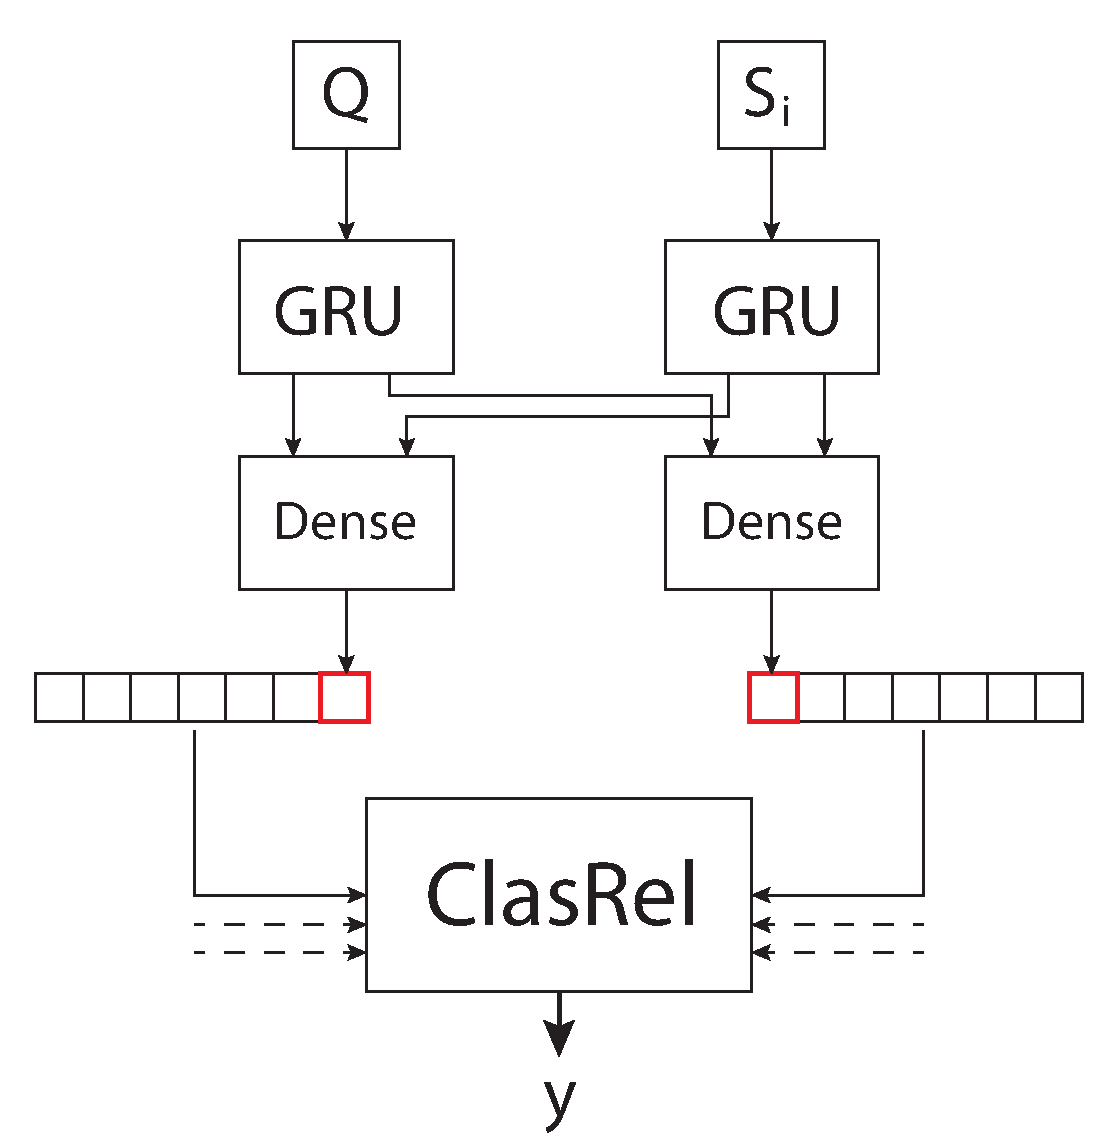
\includegraphics[width=6cm]{clasrelfull}
	\caption{The full model with RNN included.}
	\label{fig:clasrelfull}
\end{figure}

At a high level,%
\footnote{Details of the operation are described in \url{http://arxiv.org/abs/1603.06127},
the model implementation has been largely reused from the \texttt{brmson/dataset-sts} project.}
the neural network processes both the question sentence and the evidence sentence
(with GloVe word embeddings at the input rather than raw words)
and produces an aggregate numerical vector for each of the sentences that should summarize the sentence meaning.
For both classification and relevancy, a custom measure is trained that compares the numerical vectors and produces a single scalar value for each evidence, to be used in the respective feature vector.

As far as we know, this is the first time an RNN is used to decide a single answer for a question and a set of sentences (though the Memory Networks are superficially similar).
The RNN itself is trained jointly with the rest of the model described in Sec.~\ref{sec:clasrel}.
The text comprehension provided by the RNN is crucial to our current accuracy, and largely complementary to the other features listed above.
The model was tried separately, only as a classification feature and achieved accuracy over 78\%, a little more then all the other simple features put together (75\%).

\subsection{Accuracy Results}

TODO -- we are still revising our final testing methodology and performing noise-reduction $n$-run tests.

\subsection{Future Work}

To further improve the accuracy of our model, a larger dataset of questions will probably be necessary.
An alternative way to improve the number of samples would be to reduce the Syphon strictness,
though that might have repercussions to the system reliability as a whole
(since our dataset does not cover many apriori nonsensical or very hard questions).

An option we currently intensely investigate is reusing neural network models across tasks.
The overarching idea is that we could train a general ``text comprehension'' neural network
model on multiple tasks with large amounts of training data, then reuse this fixed model
on other tasks with only small amounts of data available (with only the final output
of the network, which is task specific, kept adaptable during training).
We have already had the first positive results with such a model transfer.



\bibliographystyle{plainnat}
\bibliography{qa}

\end{document}
